\documentclass[10pt,a4paper]{article}
\usepackage[margin=0.85in]{geometry}
\usepackage[T1]{fontenc}
\usepackage{mathptmx}
\usepackage[scaled=0.85]{beramono}
\usepackage{microtype}
\usepackage{graphicx}
\usepackage{booktabs}
\usepackage{amsmath}
\usepackage{xcolor}
\usepackage{tikz}
\usetikzlibrary{positioning,arrows.meta}
\usepackage[labelfont=bf,font=small,skip=3pt]{caption}
\usepackage{setspace}
\usepackage[hidelinks]{hyperref}
\setlength{\parskip}{2pt}
\setlength{\parindent}{1em}
\renewcommand{\arraystretch}{1.05}
\newcommand{\todo}[1]{\textcolor{red}{[TODO: #1]}}
\newcommand{\bs}{BiLSTM}

\title{\vspace{-1.2cm}\textbf{CS781 Capstone Project:\\In-House Legal Intelligence System}}
\author{Pranesh S\\Roll Number: 240771\\\texttt{pranesh24@iitk.ac.in}\\Indian Institute of Technology Kanpur (IIT Kanpur)}
\date{}

\begin{document}
\maketitle
\vspace{-0.8cm}
\begin{abstract}\small\noindent
Law firms cannot send confidential documents to external services, so we built a self-hosted legal language pipeline for seven tasks: language-model pretraining, named entity recognition, rhetorical roles, judgment prediction, statute identification, summarization and prior case retrieval. Our Phase-1 model is a 112.8M-parameter GPT-2-style decoder with a custom 32k byte-level BPE tokenizer, trained from scratch for 1{,}000 steps on streamed court, tribunal and statute text. Phases~2 and~3 continue this decoder; Phases~4 to~7 use four compact models trained afterwards on a domain-weighted mix (decoder, masked encoder, encoder--decoder and bidirectional LSTM). Each phase compares full, partial, low-rank, adapter, prompt and distillation fine-tuning. The most consistent finding is that how a long document is presented to the model matters more than the adaptation technique: multi-window and multi-chunk input gave the largest gains in judgment prediction and summarization, and a lexical baseline stayed competitive on statute identification.
\end{abstract}

\section{Competition Result}
Table~\ref{tab:official} lists the best valid score per phase together with the leaderboard rank and the number of valid submissions.
\begin{table}[h]\centering\small
\caption{Official phase scores and ranks (best valid submission per phase; scores recorded on 9 November 2026). Ranks were recorded on 9 November 2026; the last column is the date of the best submission.}\label{tab:official}
\begin{tabular}{@{}cllllll@{}}
\toprule
Phase & Task & Primary metric (value) & Rank & Valid subm. & Best on\\\midrule
1 & Legal LM pretraining & BERTScore F1 (0.7973) & 140 & 4 & 6 Oct\\
2 & Legal NER & strict macro-F1 (0.3232) & 119 & 14 & 11 Oct\\
3 & Rhetorical role prediction & macro-F1 (0.3922) & 127 & 6 & 14 Oct\\
4 & Court judgment prediction & macro-F1 (0.7455) & 51 & 7 & 26 Oct\\
5 & Legal statute identification & macro-F1 (0.4129) & 27 & 19 & 27 Oct\\
6 & Abstractive summarization & BERTScore F1 (0.8528) & 12 & 11 & 3 Nov\\
7 & Prior case retrieval & micro-F1@7 (0.3916) & 65 & 5 & 8 Nov\\\bottomrule
\end{tabular}
\end{table}
Codabench username: \texttt{p\_240771}. Total valid Codabench submissions across all phases: 66, taken from the submission counters on each phase page. We met the minimum of four distinct submissions in every phase: the counters show between 4 and 19 valid submissions per phase, and every phase has at least four distinct scores.

\section{Introduction and Problem Description}
A firm that handles confidential matters cannot rely on a hosted model, and general-purpose language models are not trained for the long, formulaic and heavily cross-referenced text of Indian judgments. The course asks for an in-house alternative built in stages. Phase~1 pretrains a compact legal language model under a 50M--300M parameter cap, without pretrained weights or external legal corpora. Phases~2--7 adapt that model to six tasks. In Phase~2 the input is a judgment and the output is a character-offset span with one of 12 entity labels, scored by strict macro-F1. In Phase~3 each sentence of a judgment receives one of 13 rhetorical roles, scored by macro-F1, separately for corporate-law (CL) and IT-law documents. In Phase~4 the input is a judgment and the output is a binary outcome, scored by macro-F1. In Phase~5 the output is a set of statute identifiers from 100 classes, scored by macro-F1. In Phase~6 the output is an abstractive summary scored by BERTScore~\cite{bertscore}, and in Phase~7 the output is seven candidate case identifiers per query, scored by micro-F1@7.

The constraints shaped most of our decisions. We had a single Kaggle T4 GPU with fp16 only and a 12-hour session limit, so every run had to be resumable and short enough to repeat. Exact span matching in Phase~2 forbids any approximation of character offsets. Phase~5 is multi-label, so a single softmax is wrong, and BERTScore in Phase~6 rewards fluent, fact-bearing text over copying. Our research questions were: how much do the tokenizer and data mix matter, whether Phase~1 transfer helps over simpler baselines, how best to feed long documents to models whose pretraining context is 512 tokens, how thresholds and decoding settings change results, and whether the cheaper adaptation techniques match full fine-tuning. We built all seven phases end to end on the official data. We did not attempt Phase~8, human legal evaluation, or any model trained on outside data. The code, with one notebook and one README per phase, is available at \url{https://github.com/Pranesh-hub/cs781-240771}.

\section{Data Analysis and Preprocessing}
\subsection{Sources and official splits}
Phase~1 uses the course corpus in four domains (Supreme Court, high courts, tribunals and acts); the raw training files total 19.2\,GB, of which high courts are 10.7\,GB, tribunals 6.5\,GB, Supreme Court 1.3\,GB and acts 0.7\,GB. After deduplication the corpus has 3{,}356{,}594 documents, which we split with a fixed seed into 3{,}020{,}655 training, 168{,}665 validation and 167{,}274 test documents. Phases~2--7 come from the gated Hugging Face dataset \texttt{Exploration-Lab/CS-781-Capstone}; the benchmark IL-TUR~\cite{iltur} consolidates closely related Indian legal tasks, and the individual tasks have earlier corpora for named entities~\cite{lner}, rhetorical roles~\cite{rr}, judgment prediction~\cite{ildc} and statute identification~\cite{lesicin}. Phase~2 has three folds of 35 documents each (fold~1 for training, fold~2 for validation, fold~3 for test). Phase~3 has, per domain, 40 training, 5 development and 5 test documents. Phase~4 has 37{,}387 training, 1{,}988 development and 1{,}517 test cases. Phase~5 has 42{,}750, 10{,}181 and 13{,}019 cases. Phase~6 has 7{,}030 training and 100 test documents and no development split. Phase~7 has separate query and candidate pools for each split.

\subsection{Corpus statistics that informed design}
Table~\ref{tab:data} and Figures~\ref{fig:dataA} and~\ref{fig:dataB} summarize the statistics we computed from the official files.
\begin{table}[h]\centering\footnotesize
\caption{Measured dataset statistics. ``Words'' are whitespace-separated tokens.}\label{tab:data}
\begin{tabular}{@{}lp{12.3cm}@{}}
\toprule
Phase & Statistic\\\midrule
1 & Estimated from a sample of 380--600 documents per source, tokenised with our tokenizer. High courts: 10.7\,GB, about 2.7B tokens (60\% of the corpus); tribunals: 6.5\,GB, 1.3B (30\%); Supreme Court: 1.3\,GB, 0.28B (6\%); acts: 0.7\,GB, 0.16B (3.5\%). Median (90th percentile) words per document: high courts 129 (778), tribunals 503 (4{,}015), Supreme Court 3{,}283 (8{,}787), acts 3{,}016 (14{,}647). The 3{,}000 most frequent word types overlap least between high courts and acts (Jaccard 0.34) and most between the Supreme Court and tribunals (0.50), so the sources differ in vocabulary. The training mix of the four later models (30\% Supreme Court, 30\% tribunals, 35\% high courts, 5\% acts) raises the Supreme Court share almost fivefold and lowers the high-court share by 40\%; the 393M tokens seen by the encoder are under 9\% of the corpus. Encoder validation loss by source: Supreme Court 1.592, high courts 1.679, acts 1.517, tribunals 2.187.\\
2 & Folds 1/2 hold 4{,}120/4{,}273 spans (mean 118/122 per document; documents average 31{,}400/31{,}900 characters). Frequent labels: DATE 813, PREC 624, STAT 525, AUTH 535, COURT 455, CASENO 423 (fold~1). Rare labels: WIT 67, A.COUNSEL 70, R.COUNSEL 87, JUDGE 123, RESP 191, APP 207. Median span length is 10--15 characters, except PREC (31) and CASENO (20). There are no nested or overlapping spans; 103 (fold~1) and 43 (fold~2) pairs of spans touch or are one character apart.\\
3 & CL: 10{,}593 training sentences (mean 32.7 words); Fact 28\% and RatioOfTheDecision 27\%, Issue only 17 sentences, no PrecedentOverruled. IT: 6{,}252 sentences (mean 35.3 words); RatioOfTheDecision 23\%, Fact 18\%, PrecedentOverruled 3 sentences. Dissent, PrecedentNotReliedUpon and PrecedentOverruled do not occur in the CL development documents (1{,}396 sentences), so macro-F1 over present classes differs from macro-F1 over all 13.\\
4 & Positive rate is 41\% in training but 50\% in development. Median length is 2{,}192 words in training and 2{,}822 in development. The last outcome keyword (dismissed, allowed, set aside, \ldots) sits at a median 84\% (training) and 75\% (development) of the way through a judgment.\\
5 & 100 statutes, none rare: the rarest has 272 training documents and the top ten statutes carry 41\% of all labels. Labels per document: mean 3.7, median 3, maximum 31; 21\% of documents have a single label. Median length is 430 words (90th percentile 2{,}766).\\
6 & Median document 3{,}128 words (mean 4{,}369, maximum 139{,}645); median reference summary 638 words; median compression ratio 0.22; length correlation 0.75. On average 57.5\% of summary word trigrams also occur in the source and 91.5\% of summary words do, so references are moderately extractive.\\
7 & Train 827 queries / 4{,}320 candidates; dev 118 / 1{,}023; test 237 / 1{,}727. Mean relevant cases per query 6.4 (train), 8.2 (dev), maximum 52 and 92. 95\% (train) and 90\% (dev) of pool documents are relevant to some query, with 1.29 and 1.06 queries per relevant document. Median query 4{,}508 words and median candidate 3{,}633 words; every query is in its own pool.\\\bottomrule
\end{tabular}
\end{table}
\begin{figure}[h]\centering
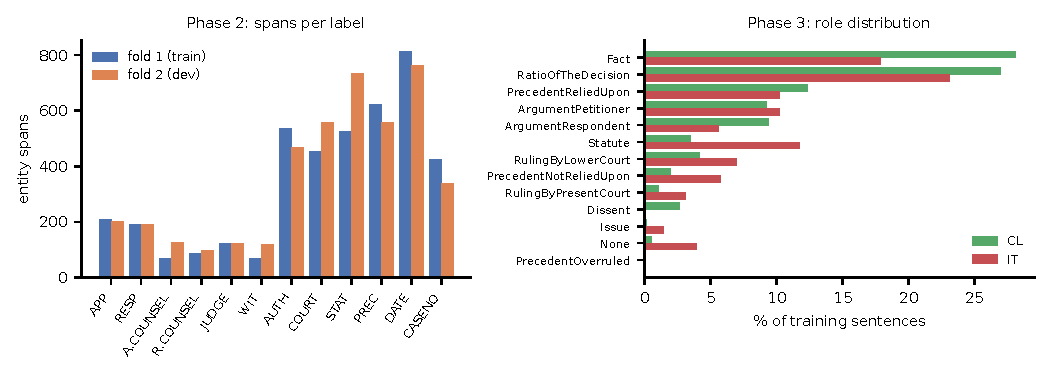
\includegraphics[width=\linewidth]{figs/fig_data_a.pdf}
\caption{Phase~2 entity spans per label in folds 1 and 2 (left) and Phase~3 role distribution in the CL and IT training sets (right).}\label{fig:dataA}
\end{figure}
\begin{figure}[h]\centering
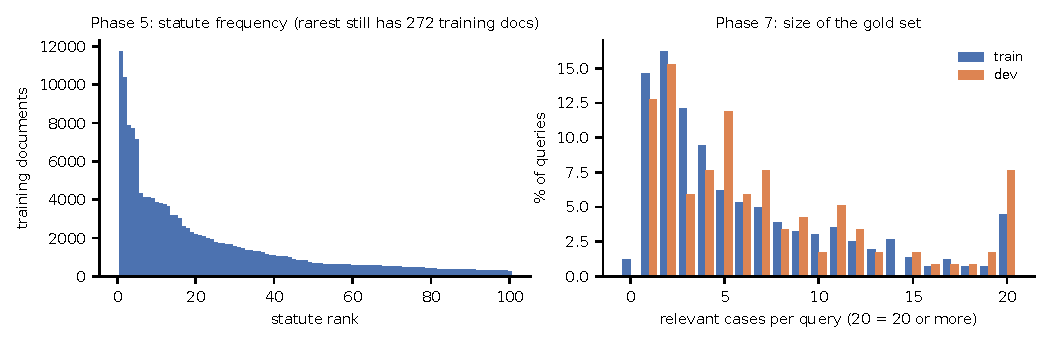
\includegraphics[width=\linewidth]{figs/fig_data_b.pdf}
\caption{Phase~5 training documents per statute (left) and Phase~7 number of relevant cases per query (right).}\label{fig:dataB}
\end{figure}
Three of these facts drove design. The shift in Phase~4 class balance (41\% to 50\%) means a threshold tuned on training-like data cannot be reused on the test set, which led to rate-matched thresholds. The near one-to-one pool in Phase~7 led to pool-aware re-ranking (Section~\ref{sec:p7}). The absence of rare statutes in Phase~5 explains why a bag-of-words baseline is so strong there. In Phase~7 the gold-set size also sets a ceiling: 59\% of development queries have fewer than seven relevant cases, so even a perfect system reaches only 0.618 micro-F1@7 on development.

\subsection{Preprocessing}
All text is tokenized with one byte-level BPE tokenizer (32{,}000 tokens plus one \texttt{[MASK]} token, so 32{,}001; PAD 0, UNK 1, BOS 2, EOS 3). The tokenizer has no decoder, which later produced generated text with spaces around punctuation (Section~\ref{sec:p6}). We do not lowercase or normalize text, because offsets must stay valid.

\emph{Phase~2.} The tokenizer returns a character offset for every token. We label a token by its overlap with a gold span (B for the first overlapping token, I for the rest) and recover spans from predicted tags by taking the first start and last end offset of each run and trimming whitespace at both ends, so predicted offsets index the original string exactly. Since gold spans never overlap, one tag per token loses nothing. \emph{Phase~3.} We use the sentence lists exactly as provided and never re-segment, so predictions align one-to-one with the official sentences; test files are stored as a mapping from document identifier to a list of sentences, unlike the labelled files. \emph{Phases~4--6.} Long documents are cut into windows of 512 tokens: the last windows first for Phase~4, up to four (eight at inference) windows, and four chunks selected by importance for Phase~6. \emph{Phase~7.} Queries and candidates use the same encoder and the same policy: up to 12 chunks of 512 tokens spread evenly over the document, each embedded as the mean of its token states and normalized.

\section{Approach and Model Evolution}
This section first describes the models we pretrained, then how they are adapted to the later tasks, and then the system of each phase. A ``window'' is a 512-token slice of a document that a classifier reads; a ``chunk'' is a slice chosen for the summarizer or the retriever.
\subsection{Phase-1 foundation model}
Our Phase-1 submission is a GPT-2-style decoder~\cite{gpt2} with 12 layers of width 768, 12 heads, learned absolute positions up to 4{,}096 tokens, pre-LayerNorm, a 3{,}072-wide GELU feed-forward block, tied embeddings and a custom vocabulary of 32{,}000 byte-level BPE tokens~\cite{bpe}, which gives 112.8M parameters. We trained it from random weights for 1{,}000 steps, with an effective batch of 8 sequences of up to 4{,}096 tokens (at most about 33M tokens), on documents streamed from the deduplicated corpus; Phases~2 and~3 continue the same model to 3{,}000 steps (about 98M tokens). For Phases~4--7 we also trained four architecture families under the 50M--300M cap (Table~\ref{tab:p1}). The second decoder is a GPT-2-style model with 12 layers of width 768, 12 heads, a 512-token context and a 3{,}072-wide GELU feed-forward block. The two decoders have the same architecture. They differ in the context length (4{,}096 against 512 position slots, which accounts for the 2.8M extra parameters of the first), in the vocabulary (the second adds one \texttt{[MASK]} token) and in the training recipe (Table~\ref{tab:p1}). The encoder is a ModernBERT-style~\cite{modernbert} masked language model with 12 layers of width 768, 12 heads, a 1{,}152-wide feed-forward block, local attention over 128 tokens with a global layer every third layer, and 30\% masking. The encoder--decoder is a T5-style~\cite{t5} model with 6+6 layers of width 640, 10 heads, gated-GELU and relative position bias, trained with span corruption. The recurrent model is two 3-layer LSTMs~\cite{lstm} of hidden size 1{,}024 (one per direction, trained with a forward and a backward language-modelling loss as in ELMo~\cite{elmo}) with 512-dimensional tied embeddings, whose concatenated states give 2{,}048-dimensional features. We verified the parameter bound by counting parameters in the saved checkpoints. The tokenizer is custom (the official one was not used), so that the vocabulary reflects legal text; the four later models add one \texttt{[MASK]} token. They were trained with the same recipe so they are comparable: sequences of 512 tokens, 131{,}072 tokens per optimizer step, and the 30/30/35/5 source mix of Section~3.2.
\begin{figure}[h]\centering
\resizebox{\linewidth}{!}{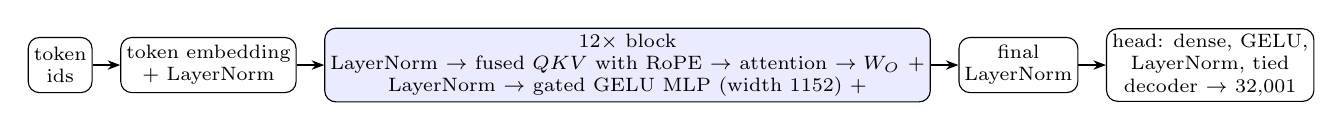
\begin{tikzpicture}[node distance=3.5mm, box/.style={draw,rounded corners,align=center,font=\scriptsize,minimum height=7mm,inner sep=2pt}]
\node[box] (in) {token\\ids};
\node[box,right=of in] (emb) {token embedding\\+ LayerNorm};
\node[box,right=of emb,fill=blue!8] (blk) {$12\times$ block\\LayerNorm $\to$ fused $QKV$ with RoPE $\to$ attention $\to W_O$ $+$\\LayerNorm $\to$ gated GELU MLP (width 1152) $+$};
\node[box,right=of blk] (fin) {final\\LayerNorm};
\node[box,right=of fin] (head) {head: dense, GELU,\\LayerNorm, tied\\decoder $\to$ 32{,}001};
\foreach \a/\b in {in/emb,emb/blk,blk/fin,fin/head} \draw[-{Stealth[length=1.6mm]}] (\a) -- (\b);
\end{tikzpicture}}
\caption{The ModernBERT-style encoder (85.4M parameters). Attention is bidirectional with rotary position embeddings; it is local (128 tokens) in all layers except every third, which is global. $+$ marks a residual connection. The decoder has the same width and depth but uses causal attention, learned absolute positions, biased LayerNorm and a 3{,}072-wide GELU MLP.}\label{fig:arch}
\end{figure}
\begin{table}[h]\centering\small
\caption{The Phase-1 decoder and the four models trained afterwards. Validation loss is not comparable across objectives.}\label{tab:p1}
\begin{tabular}{@{}llrrrrr@{}}
\toprule
Family & Objective & Params (M) & Steps & Tokens (M) & Wall-clock & Val.\ loss\\\midrule
Phase-1 decoder (4{,}096 ctx) & next token & 112.8 & 1{,}000 & $\le$33 & -- & --\\
Decoder (GPT-2 style, 512 ctx) & next token & 110.0 & 1{,}090 & 142.9 & 3.5\,h & 3.244 (ppl 25.6)\\
Encoder (ModernBERT style) & masked LM & 85.4 & 3{,}000 & 393.2 & 5.6\,h & 1.744\\
Encoder--decoder (T5 style) & span denoising & 91.3 & 1{,}520 & 199.2 & 3.4\,h & 4.838\\
\bs\ (bidirectional) & fwd + bwd LM & 63.7 & 560 & 73.4 & 1.3\,h & 5.957 (word-freq.\ 6.56)\\\bottomrule
\end{tabular}
\end{table}
The first encoder run reached a good loss but its checkpoint was lost when the session ended, so we reran it with automatic upload to a private Kaggle dataset. The \bs\ initially stalled at the unigram entropy with the usual small embedding initialization; unit-variance embeddings plus a LayerNorm before the output fixed this. Because it was trained for only 560 steps it is by far the weakest model. For the Phase~1 submission we generate with temperature 0.8 and top-$k$ 50, up to 300 new tokens, and cut each text to 128 words.

\subsection{Transfer protocol (Phases 2--7)}
Every later experiment starts from one of our own pretrained checkpoints (the Phase-1 decoder or one of the four families of Table~\ref{tab:p1}) and uses no outside weights. We attach a task head to the pretrained backbone and compare adaptation techniques: full fine-tuning, partial fine-tuning (lower layers frozen), LoRA~\cite{lora}, rank-stabilized LoRA~\cite{rslora}, the multiplicative low-rank adaptation LoRMA~\cite{lorma}, IA$^3$~\cite{ia3}, prompt tuning~\cite{prompt}, QLoRA~\cite{qlora}, Houlsby adapters~\cite{houlsby} and knowledge distillation~\cite{hinton}. Distillation always uses a half-depth student taken from the first half of the pretrained layers and a control student trained without the teacher. Figure~\ref{fig:system} shows the layout: one set of four backbones and separately fine-tuned descendants for each phase. We also fine-tuned the encoder--decoder and the \bs\ backbones in Phases~4--6. Both scored far below the encoder and the decoder (for example 0.110 against 0.393 macro-F1 for the encoder--decoder in Phase~5, and chance-level AUC for the \bs\ in Phase~4), so the final systems use the encoder and decoder families. The \bs\ has no attention layers, so adapters do not apply to it and it is only partially or fully fine-tuned. The best submission of each phase used the following backbones. Phase~1: the 1{,}000-step decoder. Phases~2 and~3: the same decoder after 3{,}000 steps (in Phase~2 followed by the rule layers). Phase~4: the fine-tuned encoder and decoder, combined into one ensemble. Phase~5: an ensemble of eight encoder runs. Phase~6: the encoder together with the decoder. Phase~7: the encoder as a bi-encoder, together with BM25 in the hybrid.
\begin{figure}[h]\centering
\resizebox{\linewidth}{!}{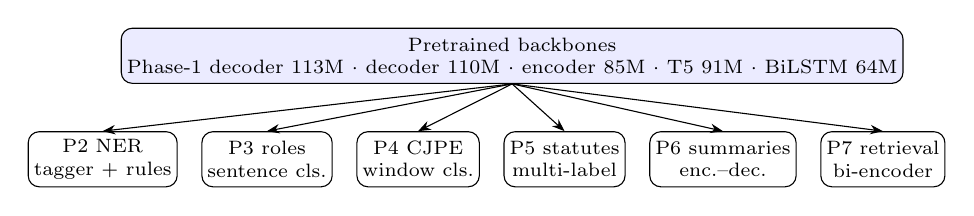
\begin{tikzpicture}[node distance=3mm, box/.style={draw,rounded corners,align=center,font=\scriptsize,minimum height=7mm,inner sep=2pt}]
\node[box,fill=blue!8] (p1) {Pretrained backbones\\Phase-1 decoder 113M $\cdot$ decoder 110M $\cdot$ encoder 85M $\cdot$ T5 91M $\cdot$ \bs\ 64M};
\node[box,below=6mm of p1,xshift=-5.2cm] (a) {P2 NER\\tagger + rules};
\node[box,right=of a] (b) {P3 roles\\sentence cls.};
\node[box,right=of b] (c) {P4 CJPE\\window cls.};
\node[box,right=of c] (d) {P5 statutes\\multi-label};
\node[box,right=of d] (e) {P6 summaries\\enc.--dec.};
\node[box,right=of e] (f) {P7 retrieval\\bi-encoder};
\foreach \x in {a,b,c,d,e,f} \draw[-{Stealth[length=1.6mm]}] (p1.south) -- (\x.north);
\end{tikzpicture}}
\caption{Overall system: separately fine-tuned descendants of our pretrained checkpoints.}\label{fig:system}
\end{figure}
In a single notebook that fine-tunes the \bs\ once per phase, the Phase~5 run reached macro-F1 0.1145 and the Phase~6 run BERTScore 0.8036 on 150 validation documents.

\subsection{Phase 2: Legal NER}
We use token classification with BIO tags over the 12 labels and recover offsets from the tokenizer's offset map as described above. Documents average more than 30{,}000 characters, so they are cut into windows of 512 tokens with a stride of 448, and probabilities of overlapping windows are averaged at inference. The champion tagger is the earlier Phase~1 decoder with a linear head, trained with class weights computed from training-token frequencies. Our diagnosis on fold~2 showed that the weak labels (RESP, A.COUNSEL, R.COUNSEL, WIT) sat near chance, with a mean probability on the correct tag of only 0.014--0.04, and that the mass went to PREC and to the outside tag; these are also the rarest labels in Table~\ref{tab:data}. Weighted loss, oversampling, a targeted pilot, longer fine-tuning and a name-swap augmentation were all rejected under criteria fixed in advance. What worked was a disclosed rule layer applied after the model, with per-label confidence thresholds on the model's spans. A counsel rule finds honorific-introduced names and assigns appellant or respondent side from nearby cue words, from the header and from the previous mention, with a default chosen on fold~1 only. JUDGE rules match header patterns such as ``Justice $X$'' and ``$X$, J.'', keeping a pattern only if its fold-1 precision was at least 0.4 with at least five true positives. Overlaps between rule spans and model spans are resolved in favour of the rules.

\subsection{Phase 3: Rhetorical role prediction}
Each sentence is encoded together with its three preceding and one following sentence (the context-aware variant) or alone (the sentence-only variant), and a classification head on the Phase~1 decoder predicts its role. We train CL and IT separately, because their label distributions and domains differ (Figure~\ref{fig:dataA}). We use class weights, label smoothing of 0.05 and early stopping with patience 3. Inference-time post-processing adds label-transition smoothing and per-class bias terms; both are tuned on the same development documents, so we treat the resulting gains with caution.

\subsection{Phase 4: Court judgment prediction}
A judgment is represented by up to four 512-token windows taken from the end (eight at inference), each encoded by the backbone and combined by a pooling head. The test threshold is rate-matched: because the dev threshold flagged 57\% of test cases while the training positive rate is 41\% and the development rate 50\% (Table~\ref{tab:data}), we choose the test threshold so that the predicted positive share matches the development share.

\subsection{Phase 5: Legal statute identification}
The head is a set of independent sigmoids over 100 statutes with binary cross-entropy, trained on windows of 512 tokens. Decision thresholds are tuned on the validation split only, comparing a single global threshold, a cardinality-matched threshold (the mean number of predicted statutes per case equals the validation mean) and per-statute thresholds shrunk toward the global one, which are adopted only if they win by a margin on a two-fold estimate; every case receives at least its top-scoring statute. The final system averages the probabilities of eight encoder runs. Two stacking models over the member outputs were rejected because they scored below the plain mean. As a reference point we also trained a classical bag-of-words baseline: TF-IDF features over word unigrams and bigrams with one linear classifier per statute and thresholds tuned on the validation split. It uses no pretrained model and is not part of any submitted file.

\subsection{Phase 6: Abstractive summarization}\label{sec:p6}
Our best system is an encoder--decoder built only from our own Phase~1 weights: the ModernBERT-style encoder reads four chunks of 512 tokens chosen by importance, and the decoder is our Phase~1 GPT-2-style model with newly added cross-attention layers (227.9M parameters in total, 33.1M trainable). All Phase~1 weights are frozen; only Houlsby bottleneck adapters, inserted after every attention and feed-forward output of both the encoder and the decoder, and the new cross-attention layers are trained. Because the Phase~1 tokenizer has no decoder, early outputs contained spaces before punctuation and inside numbers; attaching a byte-level decoder to the tokenizer fixed this. Decoding is beam search with four beams, trigram blocking and duplicate-sentence removal.

\subsection{Phase 7: Prior case retrieval}\label{sec:p7}
We train a bi-encoder on the Phase~1 encoder. Each 512-token chunk becomes the mean of its token states, normalized to a unit vector, and a document score is the mean cosine or the best-matching chunk (chosen on dev). Training uses InfoNCE~\cite{infonce} with in-batch negatives and BM25~\cite{bm25} hard negatives, masking other relevant candidates. The key design fact is that almost every candidate belongs to a single query, so a candidate that another query matches better is probably not relevant to this one. A pool-aware re-ranking step, whose Sinkhorn~\cite{sinkhorn} settings are chosen on the training split with BM25 alone, penalizes such candidates. Doubling the chunk count from 12 to 24 gave $+0.0056$ with an interval that includes zero, so we did not adopt it.

\section{Experiments and Implementation Details}
\subsection{Compute and training protocol}
All runs used a single Kaggle T4 GPU with fp16, implemented in PyTorch~\cite{pytorch} with the Hugging Face Transformers library~\cite{wolf} (T5 in fp32, where fp16 was unstable), within sessions of at most 12 hours; Pretraining of the four later models took 1.3--5.6 hours each at 9{,}000--19{,}700 tokens per second. Because runs are killed, every notebook checkpoints to disk and uploads to a private Kaggle dataset, and rolling \texttt{latest}/\texttt{best} checkpoints avoid filling the disk. We used AdamW~\cite{adamw} with warmup and learning-rate decay, a weight decay of 0.01 in Phases~2--7, gradient clipping in Phases~1, 6 and~7, and an exponential moving average of weights in Phases~4--6 (decay 0.999). Early stopping tracked a local macro-F1 (Phase~3), validation loss or BERTScore (Phase~6) and dev micro-F1@7 (Phase~7). Table~\ref{tab:impl} lists the optimizer, loss and adaptation settings of each phase.
\begin{table}[h]\centering\footnotesize
\caption{Hyperparameters of the final model in each phase. P1--P3 use the earlier decoder. $^*$Code default; the run ledger was not saved locally. $^\dagger$As recorded for its 3{,}000-step continuation.}\label{tab:hyper}
\begin{tabular}{@{}lccccccc@{}}
\toprule
 & P1 & P2 & P3 & P4 & P5 & P6 & P7\\\midrule
Parameters (M) & 112.8 & 112.8 & 112.8 & 86.5 & 86.5$^*$ & 227.9 & 84.8\\
Trainable (M) & 112.8 & 112.8 & 112.8 & 86.5 & 86.5$^*$ & 33.1 & 30.1\\
Context (tokens) & 4096 & 512 & 3+1 sent. & $4\times512$ & $4\times512$ & $4\times512$ & $\le12\times512$\\
Peak LR & $10^{-5}$$^\dagger$ & $2\cdot10^{-5}$ & $3\cdot10^{-5}$ & $5\cdot10^{-5}$ & $5\cdot10^{-5}$$^*$ & $5\cdot10^{-4}$ & $3\cdot10^{-5}$\\
Batch $\times$ accum. & $1\times8$ & $1$--$2\times8$ & 16 & 16 & 16$^*$ & 16 docs & 8\\
Epochs / steps & 1{,}000 st. & 2--3 ep. & $\le8$ ep. & 3 ep. & 3 ep.$^*$ & 4 ep. & 1{,}039 st.\\
Dropout & 0 & 0.1 (head) & 0.1 & 0.1 (head) & 0.1 (head) & 0 & 0\\
Decoding / threshold & $T{=}0.8$, top-$k$ 50 & per-label & arg-max & rate-matched & val.-tuned & beam 4 & top-7\\\bottomrule
\end{tabular}
\end{table}

\begin{table}[h]\centering\scriptsize
\caption{Implementation details by phase: optimizer and loss, and the adaptation techniques that were run (settings in brackets). All phases use AdamW~\cite{adamw}. KD is knowledge distillation (weight 0.5, temperature 2).}\label{tab:impl}
\begin{tabular}{@{}lp{7.0cm}p{7.7cm}@{}}
\toprule
Phase & Optimizer, schedule and loss & Adaptation techniques run\\\midrule
1, encoder & $\beta=(0.9,0.95)$, weight decay 0.1, peak LR $6\cdot10^{-4}$, warm-up, constant until 70\% of the steps, then linear decay to 10\%; clipping 1.0; fp16 with a gradient scaler; masked-LM loss on 30\% of the tokens & Pretraining only\\
1, decoder & Effective batch of 8 sequences of 4{,}096 tokens, fp16; next-token cross-entropy & Pretraining only; sampling at decoding time (temperature 0.8, top-$k$ 50)\\
2 & LR $2\cdot10^{-5}$, weight decay 0.01, gradient accumulation over 8 steps, fp16 with a gradient scaler; class-weighted cross-entropy over the BIO tags & Full fine-tuning; per-label confidence thresholds; counsel and JUDGE rule layers\\
3 & Warm-up 10\%, weight decay 0.01, head LR $10^{-3}$, label smoothing 0.05, class weights, early stopping (patience 3) & Full (LR $3\cdot10^{-5}$); LoRA, QLoRA and LoRMA+ (rank 8, $\alpha=16$, LR $5\cdot10^{-4}$); IA$^3$ (LR $3\cdot10^{-3}$); prompt tuning (20 tokens, LR $10^{-2}$); KD with a 6-layer student\\
4 & Warm-up 6\%, weight decay 0.01, weight averaging (EMA 0.999), head LR $10^{-3}$, LR $3\cdot10^{-5}$ (decoder) and $5\cdot10^{-5}$ (encoder); cross-entropy on windows & Full fine-tuning (decoder and encoder); IA$^3$ (decoder); rate-matched test threshold\\
5 & Warm-up 6\%, weight decay 0.01, EMA 0.999; binary cross-entropy (an asymmetric loss was also tried) & Full fine-tuning (encoder, decoder, T5); LoRMA+; KD; mean of eight encoder runs; thresholds tuned on validation\\
6 & Warm-up 6\%, weight decay 0.01, EMA 0.999, gradient clipping; LR $5\cdot10^{-4}$ (adapters) and $5\cdot10^{-5}$ (full); cross-entropy without label smoothing & Houlsby adapters (width 64); LoRA (rank 16, $\alpha=32$); LoRMA; prompt tuning; full; KD; beam search with 4 beams\\
7 & Weight decay 0.01; InfoNCE with temperature 0.05, 8 queries per batch, 2 chunks per document, 1 BM25 hard negative; LR $2\cdot10^{-5}$ (full), $3\cdot10^{-5}$ (partial), $5\cdot10^{-4}$ (LoRMA+), $3\cdot10^{-3}$ (IA$^3$, prompt) & Full; partial; LoRMA+; IA$^3$; prompt tuning; KD; pool-aware re-ranking\\\bottomrule
\end{tabular}
\end{table}

\subsection{Local evaluation}
Phases~2 and 4 use the official development folds. Phase~3 has only five development documents per domain, so any difference below about 0.02 macro-F1 is noise; our adoption rule required a gain on both domains, but even that rests on ten documents. Phase~6 has no development split, so we hold out 10\% of the training data (at least 100 and at most 1{,}000 documents, chosen by a deterministic hash of the text) and score 400 of them with BERTScore computed with roberta-large~\cite{roberta}. Local and leaderboard numbers diverged mildly. In Phase~4 the early decoder run scored 0.6709 locally and 0.6613 on the leaderboard, the encoder runs 0.754--0.764 locally and 0.735--0.738 on the leaderboard, and the best ensemble 0.7455. Phase~5 matched almost exactly (0.4128 locally, 0.4129 on the leaderboard); Phase~6 scored higher on the leaderboard (0.8528 against 0.8499); and Phase~3 scored lower (0.3922 against 0.42 and 0.45 on the CL and IT development documents, where the post-processing had been tuned on five documents). In Phase~2 the first rule-based pipeline scored about 0.2995 on fold~2 and 0.2858 on the leaderboard, and later refinements reached 0.3232; both rule layers were tuned after reading fold-1 failures, and fold~2 was also inspected, so the local Phase~2 number is not an unbiased estimate. For Phase~4 the prior shift of Section~3.2 is a further source of divergence.

\subsection{Ablations and controlled comparisons}
We changed one factor at a time wherever the budget allowed. \emph{Window count} (Phase~4): the last window alone gives AUC 0.785 for the encoder, while four windows give 0.828 and eight give 0.833 (for the decoder, 0.771 against 0.809). \emph{Distillation}: the half-depth student with a teacher beats the same student without it by 0.057 (CL) and 0.045 (IT) macro-F1 in Phase~3 (one seed), by 0.013 in Phase~5 (0.361 vs.\ 0.348), and by 0.0015 BERTScore in Phase~6 (0.8165 vs.\ 0.8150). \emph{Decoder fix} (Phase~6): 0.8396 to 0.8499 BERTScore. \emph{Pool-aware re-ranking} (Phase~7): BM25 rises from 0.2123 to 0.4069 on dev, but the trained neural systems gain nothing (top-2 ensemble $-0.0011$). We did not run a from-scratch baseline, so we cannot claim that Phase-1 initialization itself helped; the comparisons above only rank the techniques against each other. LoRMA and distillation were run in Phases~3, 5, 6 and~7, while Phases~2 and~4 used full fine-tuning (and IA$^3$ for the Phase-4 decoder).

\section{Results}
\begin{table}[h]\centering\footnotesize
\caption{Per-phase variant comparison on local development data (primary metric); leaderboard values where recorded. All numbers are single runs.}\label{tab:results}
\begin{tabular}{@{}cllll@{}}
\toprule
Phase & Variant & Technique & Dev primary metric & Codabench\\\midrule
2 & champion + counsel + JUDGE rules (first version) & full + rules & 0.2995 & 0.2858\\
2 & final rule-based pipeline & full + rules & -- & 0.3232\\
2 & champion alone & full & 0.1586 & --\\
3 & QLoRA & QLoRA & CL 0.291 / IT 0.339 & --\\
3 & KD student / no-KD control & KD & CL 0.284 / 0.227, IT 0.328 / 0.283 & --\\
3 & LoRMA+ & LoRMA & CL 0.238 / IT 0.344 & --\\
3 & best submitted ensemble & ensemble & CL 0.421 / IT 0.450 & 0.3922\\
4 & encoder, 8 windows & full & AUC 0.833, F1 0.754 & 0.7350\\
4 & GPT-2, last 512 tokens & full & F1 0.671 & 0.6613\\
4 & ensemble / best candidate (decoder + encoder) & ensemble & AUC 0.842, F1 0.767 & 0.7455\\
5 & 8-member encoder ensemble & ensemble & 0.4128 & 0.4129\\
5 & encoder / LoRMA+ / distilled / GPT-2 / T5 & various & 0.393 / 0.371 / 0.361 / 0.358 / 0.110 & --\\
5 & TF-IDF baseline (no pretrained model; reference only) & bag of words & 0.376 & --\\
6 & final: multi-chunk encoder + decoder, beam 4 & Houlsby & BERTScore 0.8499 & 0.8528\\
6 & LoRMA / full / KD / LoRA / prompt & see text & 0.8213 / 0.8175 / 0.8165 / 0.8151 / 0.8133 & 0.8183 / 0.8162 / 0.8158 / 0.8135 / --\\
7 & partial / IA$^3$ / full / LoRMA+ / KD / prompt & see text & 0.3502 / 0.3480 / 0.3457 / 0.3446 / 0.3435 / 0.3146 & --\\
7 & rule-safe neural system / BM25 hybrid & ensemble & 0.3702 / 0.3969 & 0.3467 / 0.3916\\\bottomrule
\end{tabular}
\end{table}
\begin{figure}[h]\centering
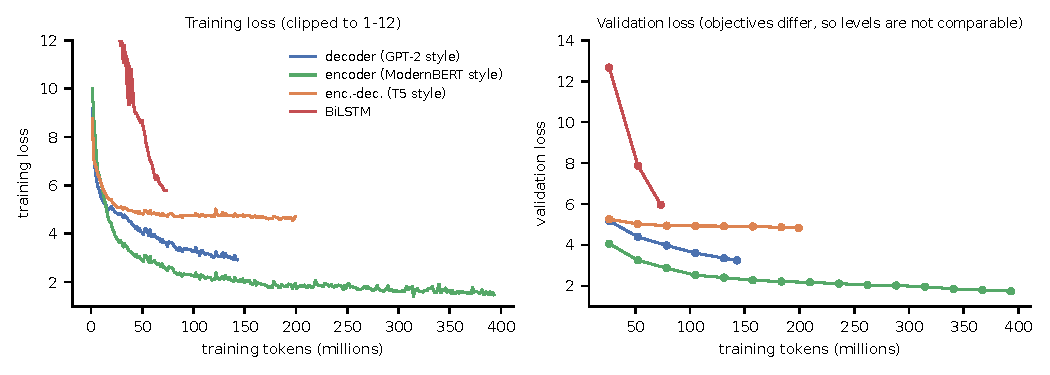
\includegraphics[width=\linewidth]{figs/fig_phase1.pdf}
\caption{Phase-1 learning curves: training loss (left) and validation loss (right) against training tokens for the four later foundation models.}\label{fig:p1}
\end{figure}
\begin{figure}[h]\centering
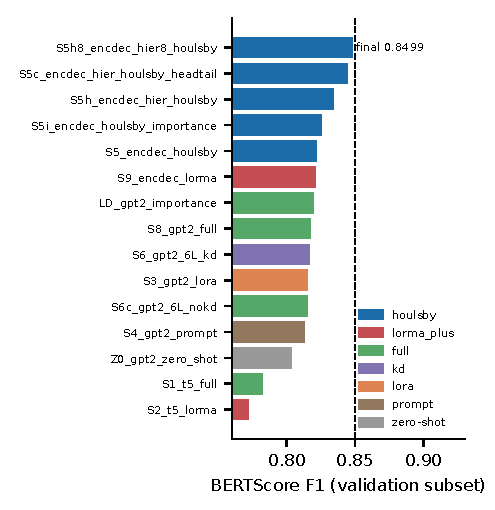
\includegraphics[width=0.48\linewidth]{figs/fig_phase6.pdf}\hfill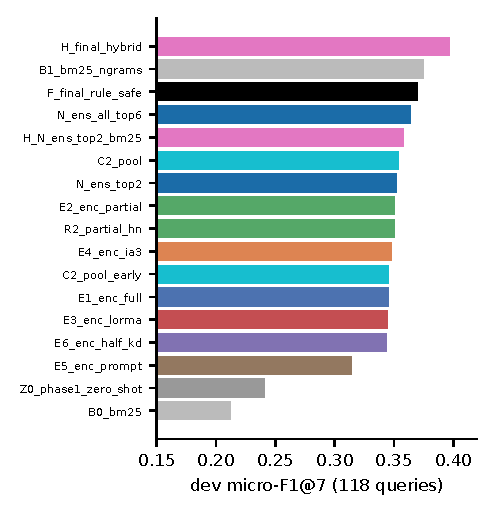
\includegraphics[width=0.48\linewidth]{figs/fig_phase7.pdf}
\caption{Left: Phase~6 BERTScore F1 per run on the 400-document held-out subset (bar colour is the technique). Right: Phase~7 development micro-F1@7 on 118 queries; the five best neural techniques are statistically tied.}\label{fig:results}
\end{figure}
Table~\ref{tab:secondary} gives the official secondary metrics of the best submission of each phase (ROUGE~\cite{rouge} in Phase~6).
\begin{table}[h]\centering\footnotesize
\caption{Official secondary metrics of the best submission in each phase (Codabench scoring output).}\label{tab:secondary}
\begin{tabular}{@{}cllll@{}}
\toprule
Phase & Primary & Secondary 1 & Secondary 2 & Note\\\midrule
1 & BERTScore F1 0.7973 & ROUGE-L 0.1782 & BLEU-4 0.0112 & 1{,}000 texts\\
2 & strict macro-F1 0.3232 & macro-P 0.3954 & macro-R 0.2902 & 35 documents\\
3 & macro-F1 0.3922 & macro-P 0.5177 & macro-R 0.3768 & 10 documents\\
4 & macro-F1 0.7455 & precision 0.7480 & recall 0.7441 & 1{,}517 cases\\
5 & macro-F1 0.4129 & micro-F1 0.5166 & subset acc.\ 0.0405 & 13{,}019 cases\\
6 & BERTScore F1 0.8528 & ROUGE-1 0.5066 & ROUGE-L 0.2634 & 100 documents\\
7 & micro-F1@7 0.3916 & micro-P@7 0.3996 & micro-R@7 0.3839 & 237 queries\\\bottomrule
\end{tabular}
\end{table}
Figure~\ref{fig:p1} shows that the encoder was still improving at the end of its 3{,}000 steps, while the decoder and encoder--decoder were stopped earlier by the time budget; none of the four had converged, which is expected at 73M--393M tokens. Figure~\ref{fig:curves} shows the metric against the epoch for Phases~3 and~4: the distilled student improves faster than its control in both domains, and the encoder stays above the decoder at every evaluation in Phase~4.

\begin{figure}[h]\centering
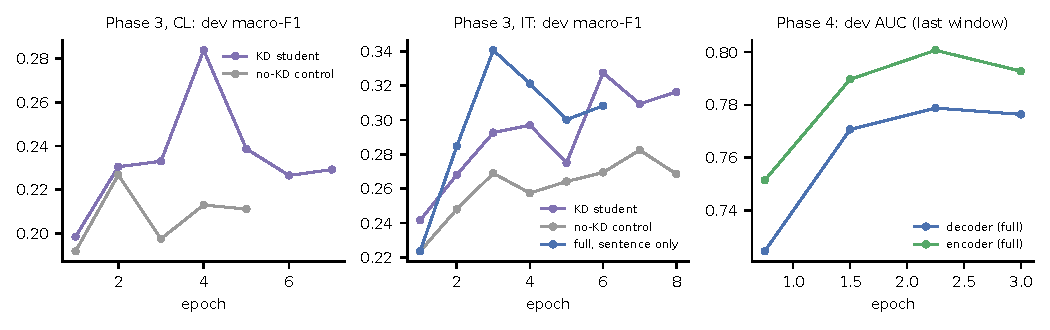
\includegraphics[width=\linewidth]{figs/fig_curves.pdf}
\caption{Metric against epoch. Phase~3: development macro-F1 of the runs logged in the final notebook (five documents per domain, so the curves are noisy). Phase~4: AUC on a 1{,}500-case development subset, scored on the last window, at four evaluation points of the three-epoch runs.}\label{fig:curves}
\end{figure}
The encoder was the best backbone in Phases~4, 5 and~7 and the encoder--decoder was best in Phase~6; Phases~2 and~3 used only the decoder. The causal reason in summarization is coverage: a 512-token input contains only 28--38\% of the reference facts, so reading four chunks raised BERTScore from 0.8217 to 0.8346, and eight chunks to 0.8485. In Phase~4 the same effect appears as the 0.04 AUC gained from extra windows, since the outcome is stated near the end. In Phase~7 the gain from the neural ensemble is limited by the one-to-one pool structure, which a re-ranking step exploits for BM25 but which trained models had apparently already absorbed. The best single adaptation technique differs by phase and the differences between techniques are within noise in Phases~3 and~7, so we do not claim a winner among them.

\section{Error Analysis and Discussion}
\subsection{Phase-wise failure modes}
\emph{Phase~2.} Official precision (0.395) exceeds recall (0.290), so the model misses entities more often than it invents them. The weak labels remain weak even after rules, because the model assigns them probability mass under PREC or the outside tag; on fold~2 the rules lift A.COUNSEL from 0.000 to 0.588, R.COUNSEL from 0.000 to 0.460 and JUDGE from 0.042 to 0.683, while RESP, WIT and APP stay near zero. These three party and witness labels have no reliable surface cue, unlike honorifics and bench headers. On fold~2 the counsel rule alone finds 95 of the 222 gold counsel spans (43\%); when it finds a span it chooses the right side 94\% of the time (89 of 95), so missed names, not the side decision, limit counsel recall, and most missed names are entries in a list of counsel without an honorific. A wrong-side case is the second name in a list ``\ldots for the petitioner Mr.\ $X$, Mr.\ $Y$, Mr.\ $Z$ \ldots for the Union of India'', where the nearest cue after the list belongs to the other party. The JUDGE rules reach precision 0.67 and recall 0.70 (85 correct of 127 predicted and 122 gold). A typical false positive is a party name in the case title, ``Justice K.S.\ Puttaswamy (Retd.)'' as a respondent, and a typical miss is a bench line in the form ``BENCH: KRISHNAIYER, V.R.''. \emph{Phase~3.} On the five CL development documents the Issue role scores F1 0.000 (3 sentences), and the best single models recover only 7--13\% of RulingByLowerCourt sentences despite a precision of 0.78--1.00; the distilled student also loses ArgumentRespondent recall (0.081 against 0.394 for the full model). The class-bias refinement improved only two of five CL documents and worsened three, so the pooled gain reflects document mix. \emph{Phase~4.} The dev threshold flagged 57\% of test cases against a 50\% development rate, which is why we rate-match the test threshold; the encoder files scored 0.735--0.738 on the leaderboard against 0.754--0.764 locally. \emph{Phase~6.} On the official test set our summaries average 382 words (44 to 472) against 932 for the references, so length is the main limitation. On the 400 held-out documents the best pre-fix system writes a median 59\% of the reference length, and 40.5\% of its summaries are shorter than half the reference; 75.5\% end in the middle of a sentence because the decoder has a 512-position limit (69 of 100 test summaries). Mean fact coverage is only 0.316, and the generated decision agrees with the reference decision in 62.6\% of the 310 documents where one can be extracted, against 36.8\% for plain GPT-2. BERTScore falls with reference length (correlation $-0.30$): the worst tenth of documents have references of 2{,}597 words on average against 459 for the best tenth. A typical GPT-2 failure is repetition, for example ``directing the Regional Regional Transport Authorities''; 44 of its 400 summaries contain an immediately repeated word. \emph{Phase~7.} The ceiling is 0.618 on development, and our best system reaches 0.397 with a lexical component or 0.370 without one (0.3916 and 0.3467 on the leaderboard), so most of the remaining gap is ranking error, not the gold-set size. \emph{Phase~5.} The official micro-F1 (0.517) is well above the macro-F1 (0.413), so frequent statutes are handled better than rare ones, and the subset accuracy of 0.040 shows that predicting the complete statute set of a case is rare when a case has 3.7 statutes on average. We did not keep per-statute outputs, so we cannot report statute-level errors.

\subsection{What the metrics do not measure}
BERTScore and ROUGE reward similarity to one hidden reference, not legal correctness: a summary can invert a holding and still score well. Strict span-F1 rewards offset perfection, so a correctly typed entity with a boundary one word off counts as both a false positive and a false negative. Micro-F1@7 treats every relevant case equally, though a firm cares about the few leading precedents. In deployment, none of these scores would replace review by a lawyer.

\subsection{Limitations and what we would do next}
The foundation models saw little data (33M--393M tokens, one to six hours each) and the \bs\ only 560 steps. Contexts of 512 tokens force chunking of documents that run to thousands of tokens, and there is no human legal evaluation. We train each phase separately, so we have not measured error propagation across a pipeline. Next steps are concrete: continue \bs\ pretraining to 1{,}400 steps and re-run its downstream phases, test a from-scratch baseline to measure Phase-1 transfer, add a label-wise attention head for Phase~5, and train a cross-encoder reranker for Phase~7.

\subsection{Surprising findings}
Three results contradicted our prior. A TF-IDF baseline (0.376) nearly matched the best single neural model on Phase~5 (0.393), which the absence of rare statutes helps to explain. Pool-aware re-ranking more than tripled the gain of BM25 yet added nothing to trained models. And in Phase~7 the lexical hybrid kept its development advantage on the leaderboard (0.3916 against 0.3467 for the neural-only system), which suggests that the pool structure it exploits is a property of the official data and not an artefact of our development split.

\section{Conclusion}
Two choices moved the metrics: presenting long documents with multiple windows or chunks, and exploiting known structure in the data, such as the end of a judgment in Phase~4, the near one-to-one pool in Phase~7 and rule layers for formulaic headers in Phase~2. Choosing among low-rank, adapter and prompt techniques did not move metrics beyond noise. The main lesson about training a compact legal model under a parameter and data lock is that capacity was not the bottleneck: input coverage and evaluation discipline were.

\begin{thebibliography}{99}\small
\bibitem{lorma} H.~Bihany, S.~Patel, A.~Modi. LoRMA: Low-rank multiplicative adaptation for LLMs. \emph{Findings of the ACL: ACL 2025}, pp.~10113--10133, 2025.
\bibitem{ia3} H.~Liu et al. Few-shot parameter-efficient fine-tuning is better and cheaper than in-context learning. \emph{NeurIPS}, 2022.
\bibitem{prompt} B.~Lester, R.~Al-Rfou, N.~Constant. The power of scale for parameter-efficient prompt tuning. \emph{EMNLP}, 2021.
\bibitem{qlora} T.~Dettmers et al. QLoRA: Efficient finetuning of quantized LLMs. \emph{NeurIPS}, 2023.
\bibitem{houlsby} N.~Houlsby et al. Parameter-efficient transfer learning for NLP. \emph{ICML}, 2019.
\bibitem{hinton} G.~Hinton, O.~Vinyals, J.~Dean. Distilling the knowledge in a neural network. \emph{arXiv:1503.02531}, 2015.
\bibitem{infonce} A.~van den Oord, Y.~Li, O.~Vinyals. Representation learning with contrastive predictive coding. \emph{arXiv:1807.03748}, 2018.
\bibitem{bm25} S.~Robertson, H.~Zaragoza. The probabilistic relevance framework: BM25 and beyond. \emph{Found.\ Trends Inf.\ Retr.}, 2009.
\bibitem{sinkhorn} M.~Cuturi. Sinkhorn distances: Lightspeed computation of optimal transport. \emph{NeurIPS}, 2013.
\bibitem{adamw} I.~Loshchilov, F.~Hutter. Decoupled weight decay regularization. \emph{ICLR}, 2019.
\bibitem{iltur} A.~Joshi, S.~Paul, A.~Sharma, P.~Goyal, S.~Ghosh, A.~Modi. IL-TUR: Benchmark for Indian legal text understanding and reasoning. \emph{Proc.\ ACL}, pp.~11460--11499, 2024.
\bibitem{lner} P.~Kalamkar et al. Named entity recognition in Indian court judgments. \emph{Natural Legal Language Processing Workshop}, 2022.
\bibitem{rr} P.~Kalamkar et al. Corpus for automatic structuring of legal documents. \emph{Proc.\ LREC}, 2022.
\bibitem{ildc} V.~Malik et al. ILDC for CJPE: Indian legal documents corpus for court judgment prediction and explanation. \emph{Proc.\ ACL}, 2021.
\bibitem{lesicin} S.~Paul, P.~Goyal, S.~Ghosh. LeSICiN: A heterogeneous graph-based approach for automatic legal statute identification from Indian legal documents. \emph{Proc.\ AAAI}, 2022.
\bibitem{gpt2} A.~Radford et al. Language models are unsupervised multitask learners. OpenAI technical report, 2019.
\bibitem{modernbert} B.~Warner et al. Smarter, better, faster, longer: A modern bidirectional encoder for fast, memory efficient, and long context finetuning and inference. \emph{arXiv:2412.13663}, 2024.
\bibitem{t5} C.~Raffel et al. Exploring the limits of transfer learning with a unified text-to-text transformer. \emph{J.\ Mach.\ Learn.\ Res.}, 21(140), 2020.
\bibitem{lstm} S.~Hochreiter, J.~Schmidhuber. Long short-term memory. \emph{Neural Computation}, 9(8), 1997.
\bibitem{elmo} M.~Peters et al. Deep contextualized word representations. \emph{Proc.\ NAACL}, 2018.
\bibitem{bpe} R.~Sennrich, B.~Haddow, A.~Birch. Neural machine translation of rare words with subword units. \emph{Proc.\ ACL}, 2016.
\bibitem{lora} E.~J.~Hu et al. LoRA: Low-rank adaptation of large language models. \emph{ICLR}, 2022.
\bibitem{rslora} D.~Kalajdzievski. A rank stabilization scaling factor for fine-tuning with LoRA. \emph{arXiv:2312.03732}, 2023.
\bibitem{bertscore} T.~Zhang et al. BERTScore: Evaluating text generation with BERT. \emph{ICLR}, 2020.
\bibitem{rouge} C.-Y.~Lin. ROUGE: A package for automatic evaluation of summaries. \emph{Text Summarization Branches Out}, 2004.
\bibitem{roberta} Y.~Liu et al. RoBERTa: A robustly optimized BERT pretraining approach. \emph{arXiv:1907.11692}, 2019.
\bibitem{pytorch} A.~Paszke et al. PyTorch: An imperative style, high-performance deep learning library. \emph{NeurIPS}, 2019.
\bibitem{wolf} T.~Wolf et al. Transformers: State-of-the-art natural language processing. \emph{EMNLP: System Demonstrations}, 2020.
\end{thebibliography}

\section*{LLM Usage Declaration}
\noindent\textbf{Q1.} Claude (Anthropic), used through Claude Code, and ChatGPT (OpenAI). \todo{add the ChatGPT model version if you know it}

\medskip\noindent\textbf{Q2.}
\begin{center}\small
\begin{tabular}{@{}p{4.6cm}|c|p{8.4cm}@{}}
\toprule
Part & Used LLM? & Purpose of using the LLM\\\midrule
Understanding concepts / papers & Yes & Explanations of methods such as LoRA variants, distillation and contrastive retrieval\\
Ideation / brainstorming at a high level & Yes & Suggestions of experiments and ablations\\
Debugging small ancillary snippets & Yes & Fixing errors in notebook cells\\
Plotting / visualization code & Yes & Matplotlib code for the report figures\\
Grammar / writing style of the report & Yes & The report text was drafted and edited with Claude\\
Report structure / section wording & Yes & Claude drafted the section text, following the template's checklist\\
Designing the model architecture & \todo{confirm} & \\
Hyperparameter search / tuning & \todo{confirm} & \\
Analysis of results / conclusions & Yes & Claude drafted the analysis from the saved run outputs \todo{rewrite in your own words}\\
Writing the core training / inference code & Yes & Notebook code was written with LLM assistance (Claude Code and ChatGPT), including the from-scratch Phase-1 models; the experiments were run by the student on Kaggle\\
Other & -- & --\\\bottomrule
\end{tabular}
\end{center}

\medskip\noindent\textbf{Q3.} Besides the lecture slides and the LLMs: the papers in the bibliography; the documentation of the Hugging Face Transformers, Tokenizers and Datasets libraries and of Kaggle; the IL-TUR benchmark pages; the official Phase~1 starter notebook; the capstone document; and the Codabench scoring outputs.

\medskip\noindent\textbf{Q4.} \todo{edit so that every sentence is true for you} I ran the pretraining and fine-tuning experiments on Kaggle T4 GPUs across three accounts, resumed them after session limits, and kept the outputs. I made 66 submissions on Codabench across the seven phases and compared each with its development score to decide which file to keep. I studied the data of every phase (label counts, document lengths, where the outcome sits in a judgment) and used these facts to choose windows, thresholds and chunking. In Phase~2 I examined why the party and witness labels stayed near zero, rejected weighted loss, oversampling and longer training after testing them against criteria fixed in advance, and kept the rule layers that helped on the development fold. In Phase~4 I noticed that the development threshold flagged 57\% of test cases against 50\% on development, and matched the positive rate instead. In Phase~7 I tested pool-aware re-ranking, which more than tripled the BM25 score but did not help the trained models. Two things failed. My first decoder stalled at a high loss, and I concluded that the training recipe and token budget, not the architecture, were the bottleneck. In Phase~4 the encoder--decoder with LoRA stayed at chance (AUC 0.50) and the BiLSTM, pretrained for only 560 steps, was at chance on judgment prediction, so I concluded that these backbones were too weakly pretrained and used the encoder and decoder families in the final systems. I did not run a from-scratch baseline, so I cannot claim that pretraining itself helped.

\end{document}
